% Chapter 1

\chapter{Introduction} % Main chapter title

\label{Chapter1} % For referencing the chapter elsewhere, use \ref{Chapter1} 

\lhead{Chapter 1. \emph{Introduction}} % This is for the header on each page - perhaps a shortened title

%----------------------------------------------------------------------------------------

\section{Computerized Axial Tomography}
A computerized axial tomography (CAT or CT) scan is one of the most important non-invasive medical imaging techniques, which was developed in the early 1970's by Godfrey Hounsfield and Allen Cormack (Fig: \ref{fig:prototype})\cite{Doe:2009:Online}. X-ray CT reconstructs a cross-sectional image by computing the attenuation coefficient distribution of an object from projection data, which records the relative number of photons passing through the object.

\begin{figure}[htbp]
	\centering
		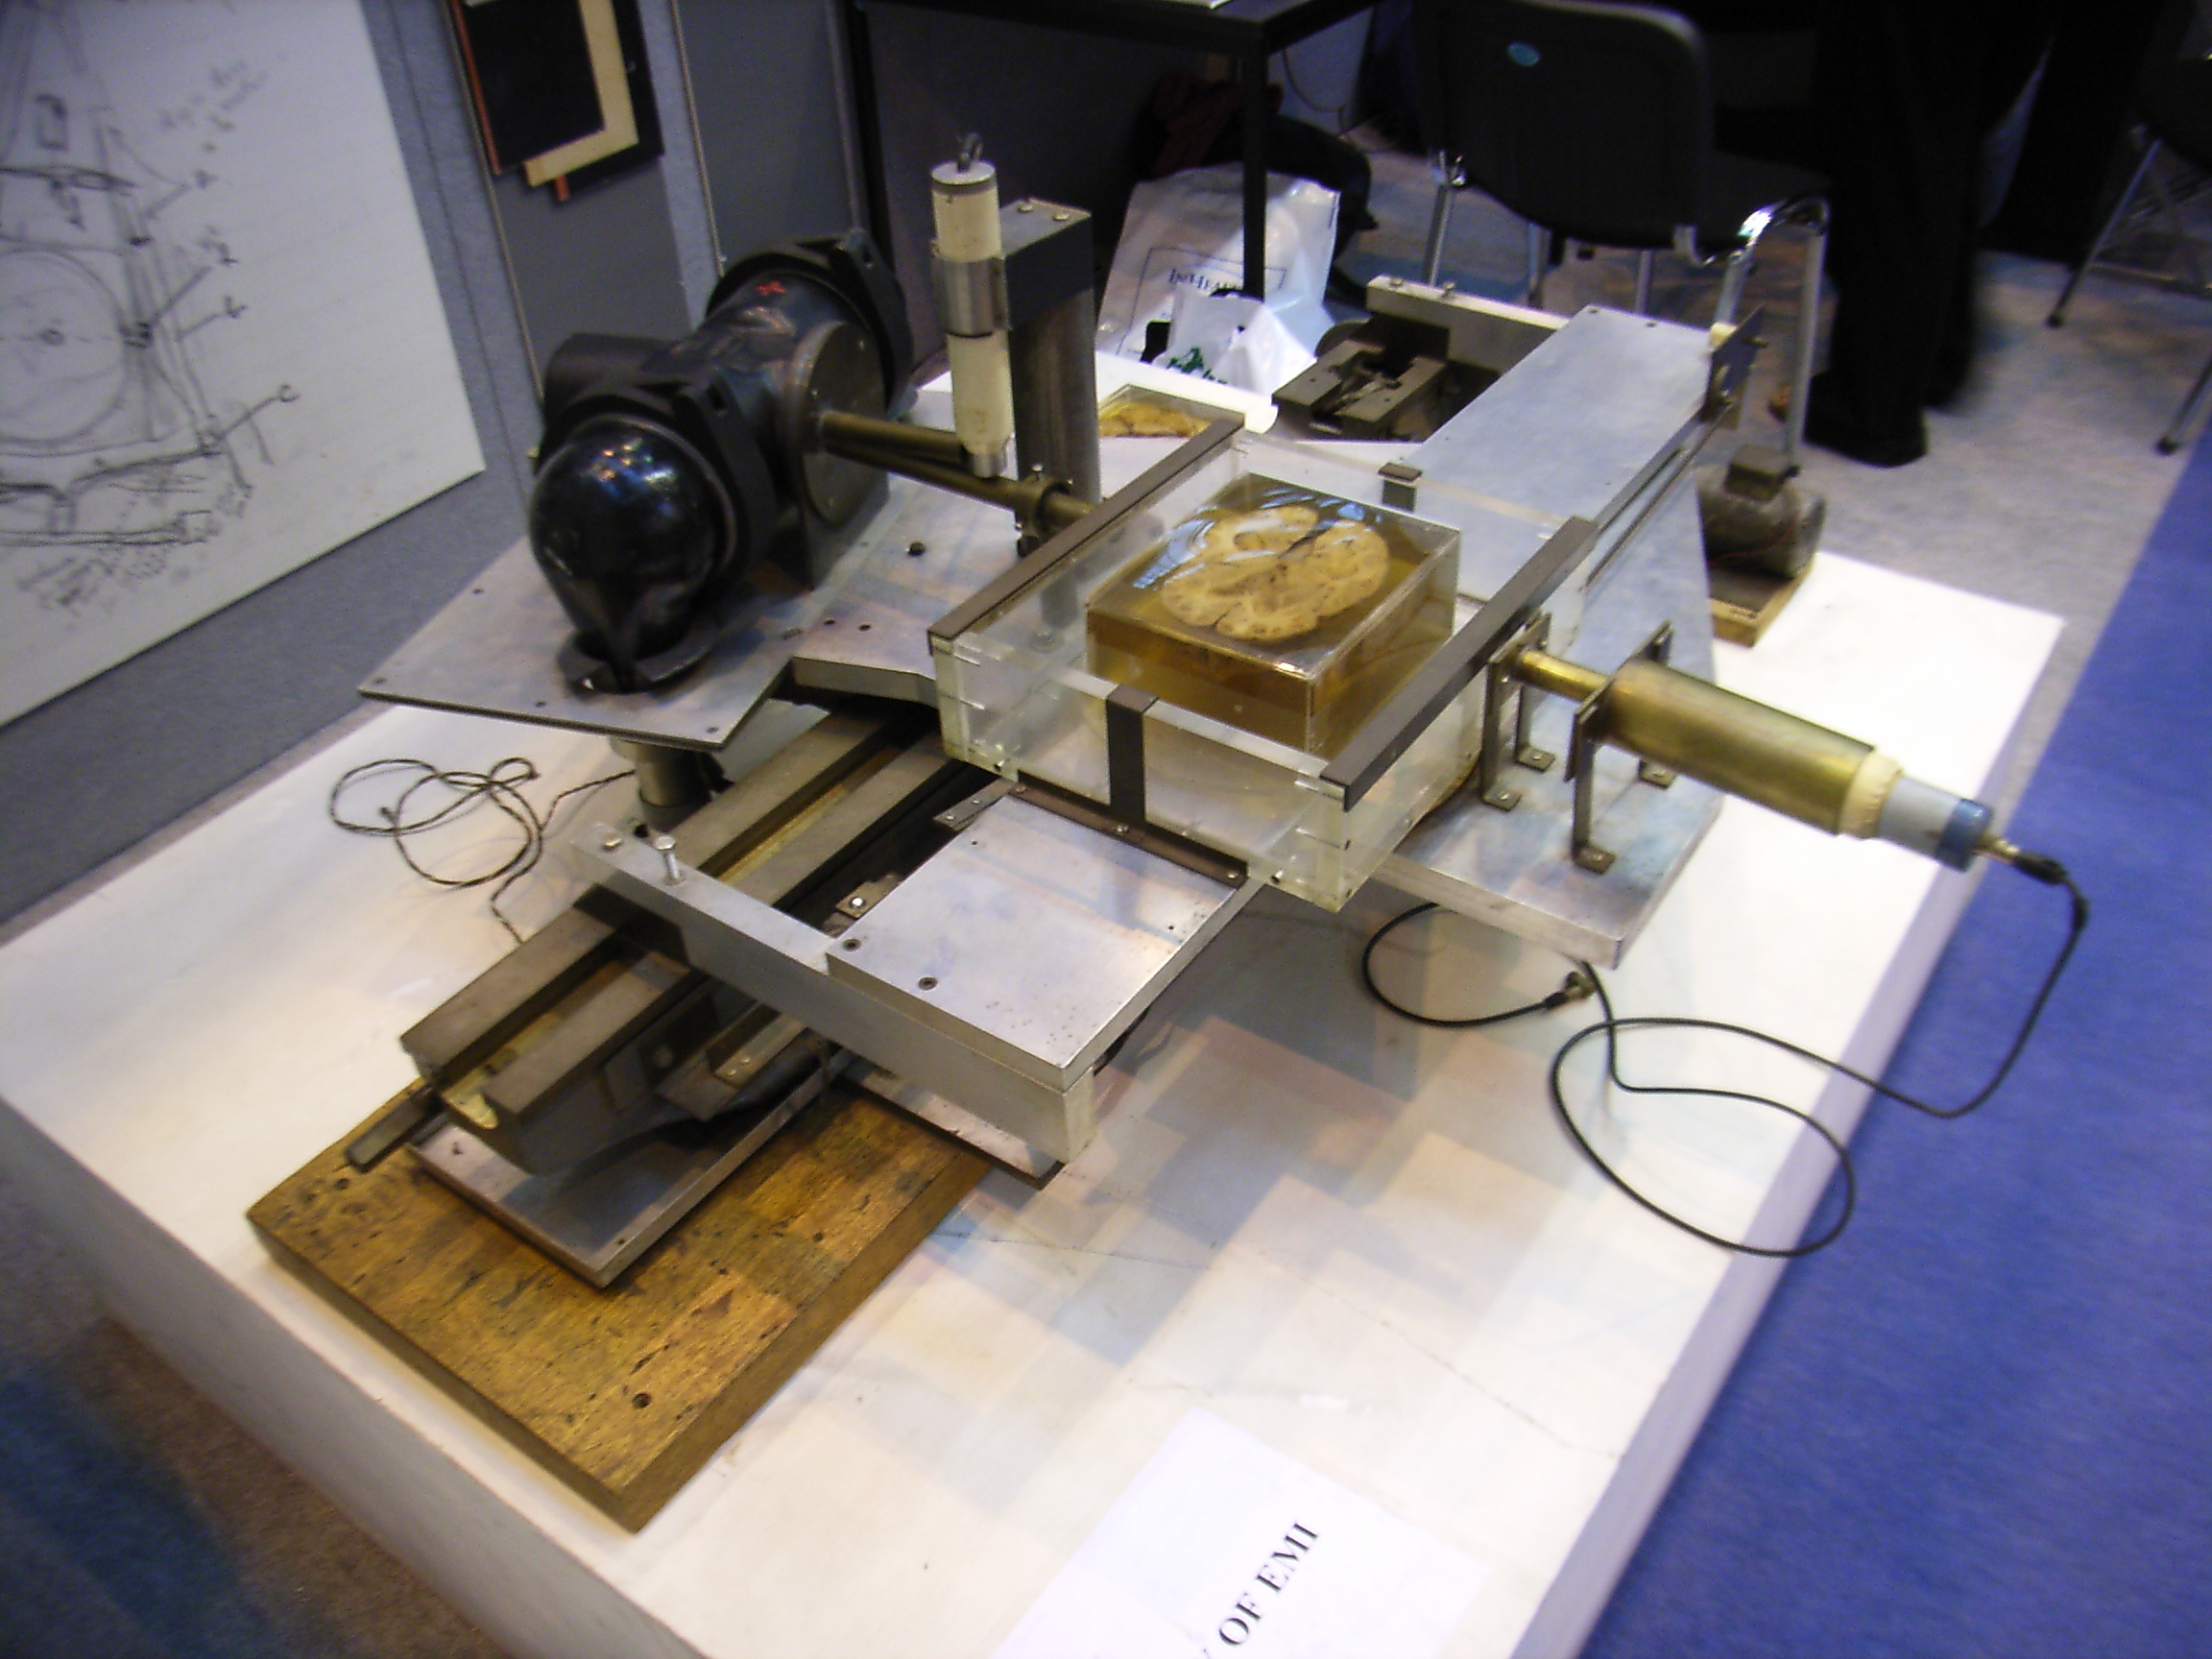
\includegraphics[width=200pt]{Figures/ct1.JPG}
	\caption[Hounsfield's prototype CT scanner]{Hounsfield's prototype CT scanner.}
	\label{fig:prototype}
\end{figure}

\section{Objective}
For the final project our team has implemented the algorithm for computerized axial tomography (CAT or CT) based on parallel beam geometry. The problem aims to solve an ill-posed inverse problem in medical imaging where X-ray beams are passed through an object and the intensity of the beams at the input and output are measured. The aim is to reconstruct an image of the internal structure of an object from the intensity variations arising from beams passing through
heterogeneous material.

Due to lack of X-ray intensity data, Shepp-Logan phantom (Fig: \ref{fig:sl}) image of the brain is used to test the reconstruction algorithm in this project. When an algorithm is applied to produce a reconstructed image of the phantom, all inaccuracies are due to the algorithm. This makes it possible to compare different algorithms in a meaningful way.   

\begin{figure}[htbp]
	\centering
		
\includegraphics[width=160pt]{Figures/Sl.png}
	\caption[Shepp-Logan Phantom]{Image of a Shepp-Logan Phantom used primarily in Tomography reconstruction.}
	\label{fig:sl}
\end{figure}


%\subsection{Figures}
%
%There will hopefully be many figures in your thesis (that should be placed in the `Figures' folder). The way to insert figures into your thesis is to use a code template like this:
%\begin{verbatim}
%\begin{figure}[htbp]
%  \centering
%    \includegraphics{Figures/Electron.pdf}
%    \rule{35em}{0.5pt}
%  \caption[An Electron]{An electron (artist's impression).}
%  \label{fig:Electron}
%\end{figure}
%\end{verbatim}
%Also look in the source file. Putting this code into the source file produces the picture of the electron that you can see in the figure below.
%
%\begin{figure}[htbp]
%	\centering
%		\includegraphics{Figures/Electron.pdf}
%		\rule{35em}{0.5pt}
%	\caption[An Electron]{An electron (artist's impression).}
%	\label{fig:Electron}
%\end{figure}

